\documentclass[12pt]{article}
\usepackage{hhline}
\usepackage{graphicx}
\graphicspath{{pictures/}}
\DeclareGraphicsExtensions{.png}
\usepackage{multirow}
\usepackage{amsmath}
\usepackage{mathtext}
\usepackage[T2A]{fontenc}
\usepackage[utf8]{inputenc}
\usepackage{pscyr} 
\usepackage[left=2cm,right=2cm, top=1.5cm,bottom=1cm,bindingoffset=0cm]{geometry}

\begin{document}
\pagestyle{empty}
\begin{center}
\large{\textbf{Университет ИТМО}}
\end{center}
\rule{500pt}{1pt}
\par\bigskip\par\bigskip\par\bigskip\par\bigskip\par\bigskip\par\bigskip\par\bigskip\par\bigskip
\begin{center}
\Large
\textbf{Отчёт по лабораторной работе №4}

\textbf{\textit{«Изучение свойств идеального газа на примере воздуха»}}


\end{center}
\par\bigskip\par\bigskip\par\bigskip\par\bigskip\par\bigskip\par\bigskip\par\bigskip\par\bigskip\par\bigskip\par\bigskip\par\bigskip\par\bigskip\par\bigskip\par\bigskip      
\begin{flushright}
\large
Выполнил: Федюкович С. А.
\par\bigskip
Факультет: МТУ “Академия ЛИМТУ”
\par\bigskip
Группа: S3100                       
\par\bigskip\par\bigskip\par\bigskip

\rule{150pt}{0.5pt}
\par\bigskip\par\bigskip\par\bigskip\par\bigskip                                                            
 Проверил: Пшеничников В. Е. 
\par\bigskip \par\bigskip

\rule{150pt}{0.5pt}
\end{flushright}
\par\bigskip\par\bigskip\par\bigskip\par\bigskip\par\bigskip\par\bigskip\par\bigskip\par\bigskip\par\bigskip\par\bigskip     
\begin{center}
\large
Санкт-Петербург
\par\bigskip
2018
\end{center}
\newpage

\section*{Цель работы}
\begin{enumerate}
\item Экспериментальная проверка уравнения состояния идеального газа.
\item Определение температуры абсолютного нуля по шкале Цельсия.
\end{enumerate}
\section*{Теоретические основы лабораторной работы}

В том случае, когда состояние  газа далеко от области фазовых превращений, его с достаточной  степенью точности можно считать идеальным. В качестве идеального газа в работе используется  обычный атмосферный воздух.

Для произвольной массы m идеального газа справедливо следующее уравнение состояния;
\begin{equation}
pV = \frac{m}{\mu}RT,
\end{equation}	 	
где $p$ --- давление, $V$ --- объем, $\mu$ --- молярная масса, $T$ --- абсолютная температура газа, $R$ --- универсальная  газовая  постоянная.
Это  уравнение  называется уравнением Менделеева-Клапейрона. 

Нулю абсолютной температуры по шкале Цельсия соответствует значение $273,15 ^{\circ}C$. Градусы шкалы абсолютной температуры (шкалы Кельвина) и шкалы Цельсия выбраны одинаковыми. Поэтому значение абсолютной температуры связано со значением температуры по шкале Цельсия формулой:
\begin{equation}
T(K) = t(^{\circ} C) - t_{o}=t(^{\circ}C)+273,15 ^{\circ}C.
\end{equation}

\begin{center}
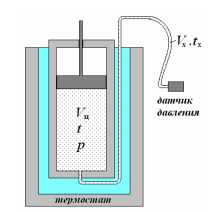
\includegraphics{1}
\end{center}
Пусть исследуемый газ находится в цилиндре с контролируемым рабочим объемом $V_{ц}$, масса газа в цилиндре $m_{ц}$. Температура $t$ цилиндра с газом поддерживается постоянной.

Датчик давления, работающий при комнатной температуре, вынесен за пределеы рабочего объёма и соединён с последним трубкой. Объём газа $V_{x}$ в этой трубке мал по сравнению с рабочим объёмом $V_{ц}$. В соединительной трубке также находится газ массой $m_{x}$ при некоторой неизвестной средней температуре $t_{x}$,  лежащей в интервале от комнатной температуры до температуры $t$ рабочего объёма.

В работе измеряется зависимость давления p газа от велечины рабочего объёма $V_{ц}$ при разных значениях температуры $t$ (от $20^{\circ} C$ до  $60^{\circ} C$). Выведем соотношение, связывающее рабочий объём и давление газа при постоянной температуре. Общее количество вещества в рабочем объёме и соединительной трубке в течение всей работы остаётся постоянным.
\begin{equation}
v = (m_{ц}+m_{x})/\mu
\end{equation}			

Выражая массы газа $m_{ц}$ и $m_{x}$ из уравнения состояния $(1)$, абсолютную температуру из соотношения $(2)$, и подставляя найденные выражения в формулу $(3)$, получим:
\begin{equation}
v = \frac{pV_{ц}}{R(t-t_{o})} +\frac{pV_{x}}{R(t_{x}-t_{o})} 
\end{equation}			
Из этого уравнения найдем искомое соотношение:
\begin{equation}
V_{ц} = \frac{vR(t-t_{o})}{p}-\frac{V_{x}(t-t_{o})}{(t_{x}-t_{o})} 
\end{equation}

Из-за перераспределения газа между объёмами $V_{ц}$ и   в процессе измерения температура   может изменяться. Однако, при относительно малой величине   изменением второго слагаемого в формуле $(5)$ можно пренебречь. Поэтому при неизменной температуре $t$ зависимость рабочего объёма $V_{ц}$ от обратного давления $1/p$ является линейной. 
\begin{equation}
K = vR(t-t_{o}),
\end{equation}

Угловой коэффициент этой зависимости в свою очередь, линейно меняется с температурой и обращается в нуль при абсолютном нуле температур. Таким образом, изучение зависимости $К(t)$ позволяет найти значение $t_{o}$.

Рассмотрим другой, более точный, способ определения величины $t_{o}$. Если для разных температур измерение давления проводить при одних и тех же значениях объёма, то полученные данные легко преобразуются в зависимость давления от температуры при разных значения рабочего объёма газа. Теоретический вид этой зависимости получается из уравнения $(5)$:
\begin{equation}
p=\frac{vR(t-t_{o})}{V_{ц}(1+x(t))}\approx \frac{vR(t-t_{o})}{V_{ц}}(1+x(t)),
\end{equation}
где $x(t)=\frac{V_{x} (t-t_{o})}{V_{ц} (t_{x}-t_{o} ) }$. Справедливость приближенного равенства в формуле (7) обусловлена тем, что значения функции $x(t)$  малы, и для малых x можно воспользоваться формулой приближенных вычислений:
\begin{equation}
(1+x)^{\alpha} \approx 1 + \alpha x.
\end{equation}
В данном случае $\alpha = -1$.

\begin{center}
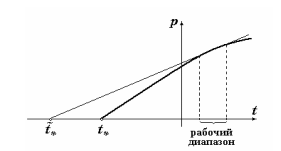
\includegraphics{2}
\end{center}
При неизменном рабочем объёме $V_{ц}$ график зависимости давления от температуры в соответствии с формулой $(7)$ должен быть почти линейным. Причем давление должно обращаться в нуль как раз при $t = t_{o}$ . Из-за малости функции $x(t)$ отклонение от линейности невилико, и при измерении в ограниченном диапазоне температур практичечки незаметно. Но, если искать значение  $t_{o}$  с помощью линейной аппроксимации экспериментальной зависимости $p(t)$, экстраполируя аппроксимирующую прямую до пересечения с осью $t$, то найденное приближенное значение   окажется систематически смещённым влево относительно истинного значения   . Причина этого в следующем. Величина $x(t)$ в первом приближении линейно растущая функция температуры, с учетом этого график функции $p(t)$ из уравнения $(7)$ оказывается параболой выпуклой вверх. Аппроксимирующая прямая, параметры которой найдены по точнкам в рабочем диапазоне температур, идет практически по касательной к этому графику, «промахиваясь» мимо истинного значения  , как изображено на рис. 1. Однако, можно показать, что разность  при малом отношении $V_{x}/V_{ц}$  должна убывать обратно пропорционально объёму $V_{ц}$. Поэтому, правильное значение температуры абсолютного нуля может быть найдено как предел:
\begin{equation}
t_{o} = \lim_{1/V_{ц}\to 0}\widetilde{t}_{o}
\end{equation}
линейным продолжением графика зависимости  $\widetilde{t}_{o}$ от $1/V_{ц}$ к значению $1/V_{ц} =0$.

\end{document}